% !TeX spellcheck = en_US
\subsection{Algorithm of the Finite Element Formulation of Heat Transfer Equation}
\begin{mdframed}
	The algorithm goes as follows:
	\begin{itemize}
		\item Discretize the domain and build the mesh.
		\item For each element $ e $ of the domain:
		\begin{itemize}
			\item Construct the Jacobian matrix $ Jac $ with the functions $ \alpha_i $
			\item Evaluate the Jacobian $ \det(Jac) $
			\item Evaluate all the 16 terms $ \nabla\alpha_i\nabla\alpha_j $ with the help of the Gauss quadrature formula.
			\item Update the global matrix $ A $ with the function \texttt{Update}
		\end{itemize}
		\item For each element $ f $ of the upper boundary:
		\begin{itemize}
			\item Construct the Jacobian $ Jac $ (that is already a scalar value) with the functions $ \alpha_1 $ and $ \alpha_2 $
			\item Evaluate all the 4 terms $ \alpha_i\alpha_j $ with the help of the 1D Gauss quadrature formula.
			\item Update the global matrix $ B $ with the function \texttt{Update} modified for the boundary elements
		\end{itemize}
		\item Solve the linear problem $ (A_{ij}+B_{ij})T_i = Q_i $
	\end{itemize}
\end{mdframed}


In the program we make use of the following functions:
\begin{itemize}
	\item \texttt{jacobian(M, Elem, e)} where \texttt{M} is the coordinates matrix and \texttt{Elem} is the mesh matrix, while \texttt{e} is the global element taken into consideration.
	\item \texttt{alpha(xi,eta)} where \texttt{xi,eta} are the local coordinates.
	\item \texttt{update} for updating the global matrix with the 16 values obtained for each element $ e $. 
	\item The functions \texttt{points} and \texttt{mesh} as already stated in Section \ref{sec:4.1} 
	\item The function \texttt{Update} for putting the values of the local matrix of each element $ e $ (resp. $ f $) in the global matrix $ A $ (resp. $ B $).
\end{itemize}


In Fig.~\ref{fig:non-coupled_thermal_problem} is plotted the 3D mesh of the non coupled solution for the Thermal Problem. 
\begin{figure}[htbp]
	\centering
	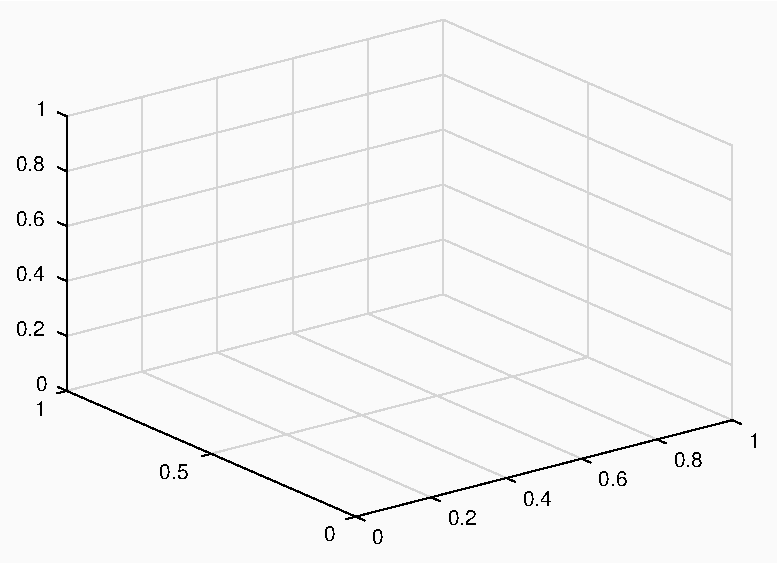
\includegraphics{Matlab_Code/Temperature_result}
	\caption{Result for the non-coupled thermal problem}
	\label{fig:non-coupled_thermal_problem}
\end{figure}



\subsection{Programming and calculation}
\subsubsection{Construct the program: main program and functions}
In the following we paste the code used in the resolution of the thermal problem. 
Listing \ref{main} is the \texttt{main} file used for the resolution. In the middle we've used several different functions, that are listed below.

\lstinputlisting[label={main},caption={main program}]{Matlab_Code/main.m}

Where we used the function \texttt{jacobian}, \texttt{alpha}, \texttt{update} and \texttt{dIntegral} listed below.

\lstinputlisting[label={jacobian},caption={function for the creation of the jacobian matrix for each element}]{Matlab_Code/jacobian.m}

\lstinputlisting[label={alpha},caption={Function for the creation of the alpha functions and the derivatives of the latter}]{Matlab_Code/alpha.m}
 
\lstinputlisting[label={update},caption={Function for update the global matrix with the values obtained for the local element $ e $}]{Matlab_Code/Update.m}

\lstinputlisting[label={dIntegral},caption={Function for evaluating the double integral$ \iint\nabla\alpha_i\nabla\alpha_j $}]{Matlab_Code/double_integral.m}

